\documentclass[12pt,spanish]{article}
\usepackage[utf8]{inputenc}
\usepackage{babel}
\usepackage{listings}
\usepackage{mathpazo}
\usepackage{enumitem}
\usepackage{courier}
\usepackage{textcomp}
\usepackage{xcolor}
\usepackage{parskip}
\usepackage{fullpage}
\usepackage{graphicx}
\usepackage{verbatim}

\newcommand{\onelinerule}{\rule[2.3ex]{0pt}{0pt}}
\newcommand{\twolinerule}{\rule[6.2ex]{0pt}{0pt}}
\newcommand{\respuesta}{\framebox[\textwidth]{\twolinerule}}
\newcommand{\nombre}{%
  \begin{tikzpicture}[xscale=.4,yscale=.7]
    \draw (0, 0) rectangle (22, 1);
  \end{tikzpicture}%
}
%\newcommand{\rol}   {\framebox[0.3\textwidth]{\onelinerule}}
\newcommand{\rol}{%
  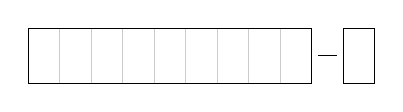
\begin{tikzpicture}[xscale=.4,yscale=.7]
    \draw[gray!40] ( 0, 0) grid      ( 9, 1);
    \draw          ( 0, 0) rectangle ( 9, 1);
    \draw          (10, 0) rectangle (11, 1);
    \draw (9 + .2, .5) -- (10 - .2, .5);
  \end{tikzpicture}%
}
\newcommand{\li}{\lstinline}
\providecommand{\pond}[1]{[{\small\textbf{#1\%}}]}

\lstdefinelanguage{py}{%
  classoffset=0,%
    morekeywords={%
      False,class,finally,is,return,None,continue,for,lambda,try,%
      True,def,from,nonlocal,while,and,del,global,not,with,print,%
      as,elif,if,or,yield,assert,else,import,pass,break,except,in,raise},%
    keywordstyle=\color{black!80}\bfseries,%
  classoffset=1,
    morekeywords={int,float,str,abs,len,raw_input,exit,range,min,max,%
      set,dict,tuple,list,bool,complex,round,sum,all,any,zip,map,filter,%
      sorted,reversed,dir,file,frozenset,open,%
      array,zeros,ones,arange,linspace,eye,diag,dot},
    keywordstyle=\color{black!50}\bfseries,%
  classoffset=0,%
  sensitive=true,%
  morecomment=[l]\#,%
  morestring=[b]',%
  morestring=[b]",%
  stringstyle=\em,%
}

\lstdefinelanguage{testcase}{%
  moredelim=[is][\bfseries]{`}{`},%
  backgroundcolor=\color{gray!20},%
}

\lstdefinelanguage{file}{%
  frame=single,%
}

\lstset{language=py}
\lstset{basicstyle=\ttfamily}
\lstset{columns=fixed}
\lstset{upquote=true}
\lstset{showstringspaces=false}
\lstset{rangeprefix=\#\ }
\lstset{includerangemarker=false}

\newlist{certamen}{enumerate}{1}
\setlist[certamen]{%
  label=\arabic*.,
  font=\LARGE\bfseries,%
  labelindent=-.5in,%
  leftmargin=0pt,%
  labelsep=1em%
}



\lstset{language=file,frame=single}

\begin{document}
  \thispagestyle{empty}
  \section*{Lunes 12 de noviembre}

  La Universidad Vecinal Ximena Yáñez Zapata
  mantiene los datos de sus ramos en archivos de texto,
  en los que cada línea corres\-ponde a un estudiante
  y contiene varios datos separados por dos puntos («\verb+:+»)
  como en el siguiente ejemplo:
  \begin{verbatim}Martin:Soto:M:1990/8/24:39,86,22,56,30\end{verbatim}

  Los datos de cada estudiante son, en orden:
  el nombre, el apellido,
  el sexo (\verb+M+ si es masculino y \verb+F+ si es femenino),
  la fecha de nacimiento (en formato \texttt{año/mes/día})
  y las notas obtenidas (separadas por comas).

  El archivo \texttt{progra.txt} contiene los datos
  de los alumnos de la asignatura de Programística.

  \begin{enumerate}[leftmargin=0pt]

    \item
      \begin{minipage}[t]{.5\textwidth}
        \parskip=2ex
        Escriba el programa \texttt{pagina\_web.py}
        que genere el archivo \texttt{progra.html},
        cuyo contenido sea como el mostrado a la derecha.
        (Por brevedad aquí sólo se muestra los primeros dos estudiantes;
        usted debe agregarlos todos).
        Los datos listados son:
        el nombre completo,
        las notas de los cinco certámenes
        y el promedio final (encerrado entre \verb+<b>+ y \verb+</b>+).

        El archivo generado es una página web.
        Al abrirlo en su navegador favorito,
        usted debería ver algo como esto:
        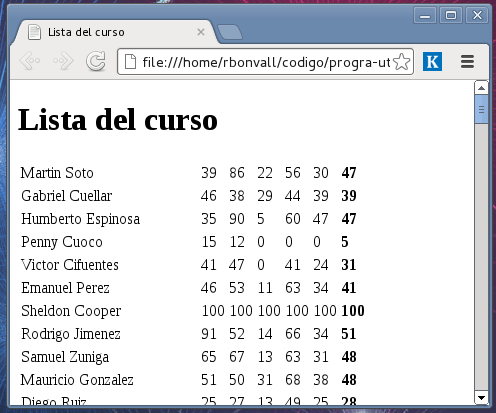
\includegraphics[width=\textwidth]{pagina.png}

      \end{minipage}
      \hfill
      \begin{minipage}[t]{.45\textwidth}
        Archivo \texttt{progra.html}:
        \lstinputlisting[basicstyle=\small\ttfamily]{ejemplo.html}
      \end{minipage}

    \newpage
    \item
      El profesor Rogelio Bombal de la asignatura de Programística
      desea enviar al término del semestre
      un email a cada estudiante para comunicarle su situación final.

      Su equipo debe escribir el programa \verb!mails.py!
      que cree una carpeta llamada \verb!emails!,
      que contenga un archivo por cada alumno
      cuyo contenido sea el mensaje del profesor.

      Para crear la carpeta,
      use la función \li!makedirs!
      provista por el módulo \li!os!.
      Para abrir un archivo dentro de la carpeta \verb!emails!,
      debe indicar tanto la carpeta como el nombre del archivo
      separados por una barra: \li!open("emails/archivo.txt")!.

      El contenido del email debe seguir el formato del siguiente ejemplo:
      \begin{lstlisting}[language=]
De: Rogelio Bombal <r.bombal@uvxyz.cl>
Para: Ignacio Navarro <i.navarro@uvxyz.cl>

Estimado Ignacio,
le informamos que usted ha aprobado con nota final 61 :)

Saludos,
Rogelio Bombal.
      \end{lstlisting}

      Por supuesto,
      el email debe decir «aprobado» o «reprobado» según corresponda,
      y debe tratar a las damas de «estimada»
      y a los caballeros de «estimado».

      La dirección de email de un alumno está formada por
      la primera letra de su nombre, un punto («\verb+.+»)
      y el apellido sin espacios,
      todo en minúsculas y seguido de \verb+@uvwyz.cl+.
      Por ejemplo,
      la dirección de María Luisa de las Mercedes es
      \verb+m.delasmercedes@uvxyz.cl+.

      El archivo con el email debe llamarse
      \texttt{\textit{Nombre}-\textit{Apellido}.txt},
      reemplazando los espacios por guiones.
      Por ejemplo,
      el email para Rolando de la Cuadra
      debe estar en el archivo \texttt{Rolando-de-la-Cuadra.txt}.

      La carita que va después de la nota
      depende del promedio obtenido:
      \framebox{\texttt{:'(}} si es menos de 35,
      \framebox{\texttt{:(}}  si está entre 35 y 54,
      \framebox{\texttt{:)}}  si está entre 55 y 84, y
      \framebox{\texttt{:D}}  si es 85 o más.


    \newpage
    \item \emph{(Opcional, sin nota)}
      En el ejercicio de la pregunta 1,
      haga que las notas menores que 55 aparezcan en rojo,
      que los números estén alineadas a la derecha,
      que la tabla tenga bordes
      y que cada columna tenga un encabezado
      («Nombre», «N1», \dots, «N5», «Promedio»).

      Deberá investigar cómo hacerlo.

      También sería apropiado que aparezca el escudo de la UVXYZ
      al comienzo de la página.

    \item \emph{(Opcional, sin nota)}
      En el ejercicio de la pregunta 1,
      haga que las filas aparezcan ordenadas por promedio,
      de mayor a menor.

  \end{enumerate}


\end{document}

